\documentclass[french]{nakrule}

\usepackage{infoBulle}
\usepackage{yFlatTable}
\usepackage{multirow}
\usepackage{calc}

\author{Samuel Riedo \& Pascal Roulin}
\title{Space Invaders}
\subtitle{Projet intégré - Système numérique}

\makeatletter
\let\runauthor\@author
\let\runtitle\@title
\makeatother

%\definecolor{mainColor}{RGB}{255,50,50}
\definecolor{blockColor}{RGB}{255,160,160}

\begin{document}


\titleTwo[pictures/title]
\symmetricalPage
\tableofcontents
\asymmetricalPage
\clearpage

%--------------------------------------------------------------------
\chapter{Introduction}
\label{introduction}
%--------------------------------------------------------------------

\emph{Space Invaders} est un jeu vidéo d'arcade créé par Tomohiro Nishikado, paru pour
la première fois en 1978 au Japon. Il est l'un des tout premiers \emph{Shoot 'em
  up}, c'est-à-dire un type de jeux consistant à abattre un grand nombre d'ennemies en
leur tirant dessus. Le principe du jeu consiste en un vaisseau spatial attaqué
par des vagues d'aliens qu'il doit détruire en leur tirant dessus sans se faire
toucher par les tirs des aliens.

\emph{Space Invaders} connu rapidement un succès mondial et est aujourd'hui
considéré comme un grand classique de l'univers vidéoludique. Il a de ce fait
connu de nombreux ports et suites sur un grand nombre de plates-formes, vieilles
comme récentes.

\section{Super Mario Bros}
\label{sec:mario}

Dans un premier temps, nous avions souhaité reproduire \emph{Super Mario Bros}.
La première tentative pour recréer le monde 1-1 du jeu original fut de créer
toute la map en une image, puis de la stocker dans une RAM ou ROM.
Un scalling de 4 permet de drastiquement réduire le nombre de pixels à stocker,
en passant de 6400x800 pour l'image d'origine à 1600x150 pour celle que nous
utiliserons.
Ceci représentait \si{240.000} pixels à stocker. En prenant en compte qu'un pixel
fait exactement un Byte (deux bits pour la composante bleu, trois pour la rouge
et trois pour la verte), les RAM et ROM à disposition de la Spartan 6
XC6LX16-CS324 ne pouvaient pas stocker toutes ces données.

Afin de contourner ce problème, l'image de base a été divisée en 8 images plus
petites, faisant chacune 200x150 pixels, soit 30kB. Il était alors possible de
stocker une image dans une ROM/RAM, puis une deuxième dans une seconde ROM/RAM,
mais il était à nouveau impossible d'enregistrer les six suivantes sans dépasser
les capacités de la carte.

Devant ces limitations hardware, la décision fut prise de changer de jeu. Il nous
est apparu qu'avoir un font statique, ou alors une répétition permanente d'un
même arrière-plan était indispensable pour que le projet soit synthétisable sur
notre carte. Un jeu tel que \emph{Super Mario Bros}, avec des mondes très
différents et non répétitifs, n'est pas adapté à la programmation VHDL sur un
hardware limité. Notre choix s'est alors porté sur \emph{Space Invaders}.


\clearpage
\symmetricalPage

\section{Gameplay}
\label{sec:gameplay}

Space Invaders est un jeu en deux dimensions, aussi appelé jeu en 2D ou tout
simplement jeu 2D. Le joueur contrôle un vaisseau spatial pouvant se déplacer
uniquement sur l'axe $X$, et tirer des lasers vers le haut de l'écran. Il est
confronté à plusieurs aliens, se déplaçant aléatoirement dans la partie
supérieure de l'écran. Ces derniers tirent aléatoirement des lasers vers le bas
pour détruire le vaisseau spatial contrôlé par le joueur.

Si le vaisseau du joueur se fait toucher par un laser alien, la partie est
perdue. Si, au contraire, le joueur réussit à détruire tous les aliens sans se
faire lui-même toucher, il gagne la partie. La figure \ref{gameOnArcade} représente une
partie typique de \emph{Space Invaders} sur une borne arcade tel que le jeu était
lors de son lancement initial en 1978.

\begin{figure}[ht]
  \centering
  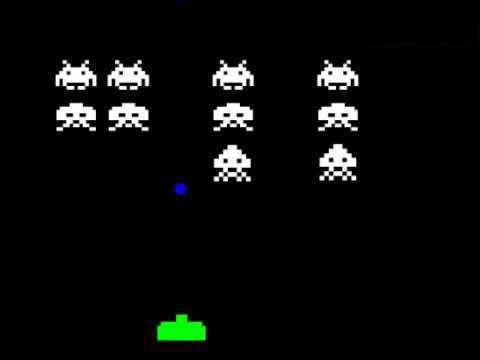
\includegraphics[width=.6\textwidth]{pictures/gameOnArcade}
  \caption{Space Invaders sur borne arcade}
  \label{gameOnArcade}
\end{figure}

Le vaisseau du joueur est représenté par la forme verte. Ce dernier à tiré un
laser, symbolisé par un point bleu. Les aliens, au nombre de 10, ont déjà été
partiellement déssimés. Au début d'une partie, leur nombre et leur disposition
forment une grille rectangulaire complète.

\infoInfo{Types d'aliens}{Bien que les aliens peuvent avoir plusieurs formes
  différentes (trois sur la figure \ref{gameOnArcade}), cela n'influence en rien
  leur comportement. Il ne s'agit ni plus ni moins que de leur apparence.}

Les versions suivantes de \emph{Space Invaders} implémenteront de nouvelles
fonctionnalités, tel que:\vspace{.1in}
\begin{items}
\item Score, déterminer par les aliens détruits et le temps pour y arriver.
\item Vaisseau alien traversant l'écran horizontalement de façon aléatoire. Le
  détruire rapport des points bonus.
\item Bouclier pour protéger le vaisseau.
\end{items}

\clearpage

\section{Déroulement d'une partie}
\label{sec:deroulementPartie}

\begin{wrapfigure}[18]{l}{.5\textwidth}
  \centering
  
\includegraphics[width=.5\textwidth]{../ROM/pictures/startScreen}
  \caption{Ecrand d'acceuil}
  \label{gameTitle}
\end{wrapfigure}

Au démarrage du jeu, un écran d'accueil est affiché (figure \ref{gameTitle}).
Lorsque le joueur presse sur le bouton central de la croix directionnelle \emph{BtnC}, la
partie commence directement. Le vaisseau du joueur est initialement positionné
au centre de l'écran sur l'axe $X$, de même que les aliens.

Au moyen des touches gauche \emph{BtnL}, droite \emph{BtnR} et haut \emph{BtnU}
de la croix directionnelle, le joueur peut respectivement déplacer son vaisseau
à gauche ou à droite, ainsi que tirer des missiles en direction des aliens pour
les éliminer. Le jeu reste dans cet état tant que le joueur ne s'est pas fait
toucher, ou qu'il y a encore des aliens en vie.

Lorsque la partie se termine, deux fins sont possibles.
Dans la première, le joueur à éliminer tous les aliens et un écran ``You Win'' est affiché, alors que le texte change
pour ``Game Over'' dans la deuxième ou il s'est fait toucher. Il est possible, à tout moment, de réinitialiser le jeu avec un reset software
en actionnant le switch \emph{SW8}.

\vspace{.1in}

\begin{figure}[h]
  \centering
  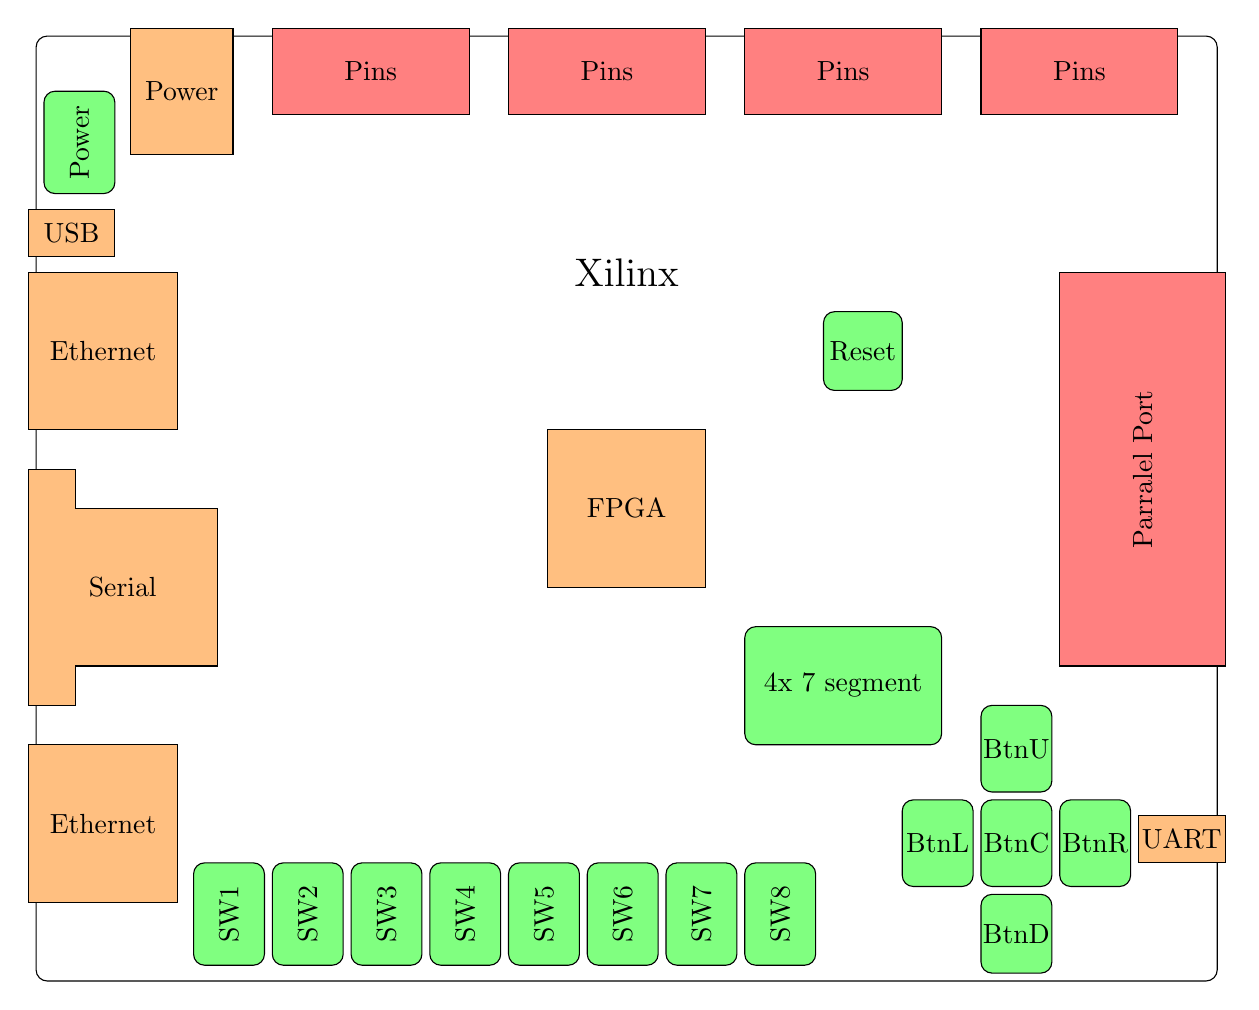
\begin{tikzpicture}
    \draw[rounded corners] (0,0) rectangle (15,12);
    % Switchs
    \draw[rounded corners, fill=green!50] (2,.2) rectangle node{\rotatebox{90}{SW1}} (2.9,1.5);
    \draw[rounded corners, fill=green!50] (3,.2) rectangle node{\rotatebox{90}{SW2}} (3.9,1.5);
    \draw[rounded corners, fill=green!50] (4,.2) rectangle node{\rotatebox{90}{SW3}} (4.9,1.5);
    \draw[rounded corners, fill=green!50] (5,.2) rectangle node{\rotatebox{90}{SW4}} (5.9,1.5);
    \draw[rounded corners, fill=green!50] (6,.2) rectangle node{\rotatebox{90}{SW5}} (6.9,1.5);
    \draw[rounded corners, fill=green!50] (7,.2) rectangle node{\rotatebox{90}{SW6}} (7.9,1.5);
    \draw[rounded corners, fill=green!50] (8,.2) rectangle node{\rotatebox{90}{SW7}} (8.9,1.5);
    \draw[rounded corners, fill=green!50] (9,.2) rectangle node{\rotatebox{90}{SW8}} (9.9,1.5);
    % Pad
    \draw[rounded corners, fill=green!50] (11,1.2) rectangle node{BtnL} (11.9,2.3);
    \draw[rounded corners, fill=green!50] (12,1.2) rectangle node{BtnC} (12.9,2.3);
    \draw[rounded corners, fill=green!50] (13,1.2) rectangle node{BtnR} (13.9,2.3);
    \draw[rounded corners, fill=green!50] (12,.1) rectangle node{BtnD} (12.9,1.1);
    \draw[rounded corners, fill=green!50] (12,2.4) rectangle node{BtnU} (12.9,3.5);

    \draw[fill=orange!50] (-.1, 1) rectangle node{Ethernet} (1.8, 3);
    \draw[fill=orange!50] (-.1, 3.5) -- (.5, 3.5) -- (.5, 4) -- (2.3, 4) -- (2.3, 6) -- (.5,6)
    -- (.5, 6.5) -- (-.1, 6.5) -- cycle;
    \node at (1.1,5) {Serial};
    \node at (7.5,9) {\Large Xilinx};
    \draw[fill=orange!50] (-.1, 7) rectangle node{Ethernet} (1.8, 9);
    \draw[fill=orange!50] (-.1, 9.2) rectangle node{USB} (1, 9.8);
    \draw[rounded corners, fill=green!50] (.1,10) rectangle node{\rotatebox{90}{Power}} (1,11.3);
    \draw[fill=orange!50] (1.2, 12.1) rectangle node{Power} (2.5, 10.5);
    \draw[fill=red!50] (3, 12.1) rectangle node{Pins} (5.5, 11);
    \draw[fill=red!50] (6, 12.1) rectangle node{Pins} (8.5, 11);
    \draw[fill=red!50] (9, 12.1) rectangle node{Pins} (11.5, 11);
    \draw[fill=red!50] (12, 12.1) rectangle node{Pins} (14.5, 11);

    \draw[fill=red!50] (15.1, 9) rectangle node{\rotatebox{90}{Parralel Port}} (13, 4);
    \draw[fill=orange!50] (15.1, 1.5) rectangle node{UART} (14, 2.1);
    % FPGA
    \draw[fill=orange!50] (6.5, 5) rectangle node{FPGA} (8.5, 7);
    % Reset
    \draw[rounded corners, fill=green!50] (10,7.5) rectangle node{Reset} (11,8.5);
    % 7 segments
    \draw[rounded corners, fill=green!50] (9,3) rectangle node{4x 7 segment} (11.5,4.5);
  \end{tikzpicture}
  \caption{Digilent NEXYS 3}
  \label{motherboard}
\end{figure}



% --------------------------------------------------------------------
\asymmetricalPage
\chapter{Architecture}
\label{architecture}

La réalisation du projet fut divisée en 6 principaux blocs, plus un top module et
un package. Trois de ces blocs furent repris du travail pratique concernant
l'affichage par VGA, alors que les autres ont été spécialement implémentés pour
ce projet.

Le fait d'avoir déjà une base de départ nous a poussé à implémenter le jeu
fonction par fonction, puis de tester et déboguer chaque nouvel ajout dès qu'il
fut coder. Cette approche présente l'avantage, contrairement à un développement
de chaque composant indépendamment les uns des autres, de réduire le risque
d'incompatibilité entre deux composants afin que le lourd travail de
débogage final soit réduit. En revanche, cette technique ne permet pas de répartir
efficacement le travail dans une équipe constituée de nombreuses personnes.

Bien que nous puissions tester le bon fonctionnement de chaque bloc et fonction
directement en programmant la FPGA pour voir le résultat sur l'écran, chaque
bloc sera testé par une macro pour valider tous les cas pouvant intervenir dans
le déroulement d'une partie. De plus, deux composants, \emph{Input} et
\emph{rocketManager}, seront testé via un testbench.

\symmetricalPage

\section{alienRocket}
\label{sec:alienRocket}


\begin{wrapfigure}[21]{r}{.55\textwidth}
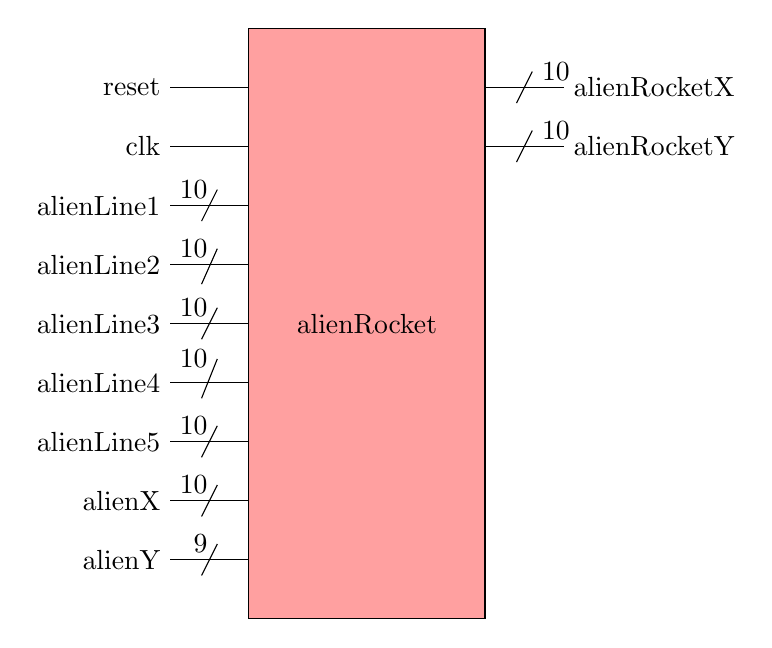
\begin{tikzpicture}
  \draw[fill=blockColor] (0,0) rectangle node{alienRocket}(3,-7.5);
  % Inputs
  \draw (-1,-.75) node[left]{reset}-- (0,-.75);
  \draw (-1,-1.5) node[left]{clk}-- (0,-1.5);
  \draw (-1,-2.25) node[left]{alienLine1}-- (0,-2.25);
  \draw (-.4,-2.05) node[left]{10} -- (-.6, -2.45);
  \draw (-1,-3) node[left]{alienLine2}-- (0,-3);
  \draw (-.4,-2.8) node[left]{10} -- (-.6, -3.25);
  \draw (-1,-3.75) node[left]{alienLine3}-- (0,-3.75);
  \draw (-.4,-3.55) node[left]{10} -- (-.6, -3.95);
  \draw (-1,-4.5) node[left]{alienLine4}-- (0,-4.5);
  \draw (-.4,-4.2) node[left]{10} -- (-.6, -4.7);
  \draw (-1,-5.25) node[left]{alienLine5}-- (0,-5.25);
  \draw (-.4,-5.05) node[left]{10} -- (-.6, -5.45);
  \draw (-1,-6) node[left]{alienX}-- (0,-6);
  \draw (-.4,-5.8) node[left]{10} -- (-.6, -6.2);
  \draw (-1,-6.75) node[left]{alienY}-- (0,-6.75);
  \draw (-.4,-6.55) node[left]{9} -- (-.6, -6.95);
  % Outputs
  \draw (4,-.75) node[right]{alienRocketX}-- (3,-.75);
  \draw (3.6,-.55) node[right]{10} -- (3.4, -.95);
  \draw (4,-1.5) node[right]{alienRocketY}-- (3,-1.5);
  \draw (3.6,-1.3) node[right]{10} -- (3.4, -1.7);
\end{tikzpicture}
\caption{Schéma bloc}
\label{alienRocketBloc}
\end{wrapfigure}

Le bloc \emph{alienRocket} gère les roquettes, aussi appelé laser ou missile, tirées par
les aliens en direction du spationef. Il est chargé de générer de nouveaux
missiles ainsi que de transmettre les informations nécessaires au bloc \emph{Display} pour afficher
correctement une roquette à l'écran.
Dans notre implémentation du jeu, le joueur fait face à 50 aliens, réparties en
une grille de 5 lignes et 10 colonnes (tableau \ref{alientable}). Par colonne,
chaque alien le plus proche du bas de l'écran peut tirer une roquette vers le
bas pour tenter de détruire le vaisseau du joueur. Une seule roquette peut être
affichée à l'écran en même temps (sans compter les tirs du joueur). Cela signifie
que tant que le missile n'a pas atteint le bas de l'écran, les aliens ne peuvent
pas en tirer un nouveau.

Lorsqu'une roquette peut être tirée, le choix de la colonne d'alien pouvant tirer
se fait de manière aléatoire entre toutes les colonnes qui contiennent au moins un
alien. Par exemple, soit les aliens encore en vie selon le tableau
\ref{alientable}. Une roquette peut être tirée depuis les aliens 0-4 et 7-9 de la
ligne 5 (alienLine5), ainsi que depuis les aliens 5 et 6 de la ligne 4 (alienLine4).

\begin{table}[ht]
  \centering
  \begin{tabular}{c c c c c c c c c c c}
    & \multicolumn{10}{c}{Index}\\
    & 0 & 1 & 2 & 3 & 4 & 5 & 6 & 7 & 8 & 9 \\
    $\begin{matrix}\text{alienLine1}\\ \text{ }\end{matrix}$ & 
\includegraphics[width=.05\textwidth]{pictures/aliens/blue}&
    
\includegraphics[width=.05\textwidth]{pictures/aliens/blue}&
    
\includegraphics[width=.05\textwidth]{pictures/aliens/blue}&
    
\includegraphics[width=.05\textwidth]{pictures/aliens/blue}&
    
\includegraphics[width=.05\textwidth]{pictures/aliens/blue}&
    
\includegraphics[width=.05\textwidth]{pictures/aliens/blue}&
    
\includegraphics[width=.05\textwidth]{pictures/aliens/blue}&
    
\includegraphics[width=.05\textwidth]{pictures/aliens/blue}&
    
\includegraphics[width=.05\textwidth]{pictures/aliens/blue}&
    
\includegraphics[width=.05\textwidth]{pictures/aliens/blue}\\
    $\begin{matrix}\text{alienLine2}\\ \text{ }\end{matrix}$ & 
\includegraphics[width=.05\textwidth]{pictures/aliens/DarkBlue}&
    
\includegraphics[width=.05\textwidth]{pictures/aliens/DarkBlue}&
    
\includegraphics[width=.05\textwidth]{pictures/aliens/DarkBlue}&
    
\includegraphics[width=.05\textwidth]{pictures/aliens/DarkBlue}&
    
\includegraphics[width=.05\textwidth]{pictures/aliens/DarkBlue}&
    
\includegraphics[width=.05\textwidth]{pictures/aliens/DarkBlue}&
    
\includegraphics[width=.05\textwidth]{pictures/aliens/DarkBlue}&
    
\includegraphics[width=.05\textwidth]{pictures/aliens/DarkBlue}&
    
\includegraphics[width=.05\textwidth]{pictures/aliens/DarkBlue}&
    
\includegraphics[width=.05\textwidth]{pictures/aliens/DarkBlue}\\
    $\begin{matrix}\text{alienLine3}\\ \text{ }\end{matrix}$ & 
\includegraphics[width=.05\textwidth]{pictures/aliens/green}&
    
\includegraphics[width=.05\textwidth]{pictures/aliens/green}&
    
\includegraphics[width=.05\textwidth]{pictures/aliens/green}&
    
\includegraphics[width=.05\textwidth]{pictures/aliens/green}&
    
\includegraphics[width=.05\textwidth]{pictures/aliens/green}&
    
\includegraphics[width=.05\textwidth]{pictures/aliens/green}&
    
\includegraphics[width=.05\textwidth]{pictures/aliens/green}&
    
\includegraphics[width=.05\textwidth]{pictures/aliens/green}&
    
\includegraphics[width=.05\textwidth]{pictures/aliens/green}&
    
\includegraphics[width=.05\textwidth]{pictures/aliens/green}\\
    $\begin{matrix}\text{alienLine4}\\ \text{ }\end{matrix}$ & 
\includegraphics[width=.05\textwidth]{pictures/aliens/yellow}&
    
\includegraphics[width=.05\textwidth]{pictures/aliens/yellow}&
    
\includegraphics[width=.05\textwidth]{pictures/aliens/yellow}&
    
\includegraphics[width=.05\textwidth]{pictures/aliens/yellow}&
    
\includegraphics[width=.05\textwidth]{pictures/aliens/yellow}&
    
\includegraphics[width=.05\textwidth]{pictures/aliens/yellow}&
    
\includegraphics[width=.05\textwidth]{pictures/aliens/yellow}&
    
\includegraphics[width=.05\textwidth]{pictures/aliens/yellow}&
    
\includegraphics[width=.05\textwidth]{pictures/aliens/yellow}&
    
\includegraphics[width=.05\textwidth]{pictures/aliens/yellow}\\
    $\begin{matrix}\text{alienLine5}\\ \text{ }\end{matrix}$ & 
\includegraphics[width=.05\textwidth]{pictures/aliens/purple}&
    
\includegraphics[width=.05\textwidth]{pictures/aliens/purple}&
    
\includegraphics[width=.05\textwidth]{pictures/aliens/purple}&
    
\includegraphics[width=.05\textwidth]{pictures/aliens/purple}&
    
\includegraphics[width=.05\textwidth]{pictures/aliens/purple}&&&
    
\includegraphics[width=.05\textwidth]{pictures/aliens/purple}&
    
\includegraphics[width=.05\textwidth]{pictures/aliens/purple}&
    
\includegraphics[width=.05\textwidth]{pictures/aliens/purple}\\
  \end{tabular}
  \caption{Gestion des aliens dans le jeux}
  \label{alientable}
\end{table}

Les signaux \emph{alienLine1} à \emph{alienLine5} sont des
\emph{std\_logic\_vector} de 10 bits. Chaque bit indique par une valeur à 1 la
présence d'un alien à l'index correspondant, alors qu'un 0 indique que l'alien a
été tué par le joueur. Par exemple, selon le tableau \ref{alientable},
\emph{alienLine5} vaut \emph{1111100111}.

La fréquence à laquelle les aliens tirent des roquettes peut être modifiée en
changeant la constante \emph{rocketFrequency} dans le package \emph{SpaceInvadersPackage}.

\clearpage

\subsection{Entrées \& Sorties}
\label{subsec:Entrees_Sorties_alienRocket}

\begin{descr}
  \itemColor{reset} Reset du circuit, actif à l'état haut.
  \itemColor{clk} Horloge 40MHz, active sur front montant.
  \itemColor{alienLine1} Indique, par un 0 un alien vivant, et par 1 un alien
  mort dans la ligne d'alien de la partie supérieure de l'écran.
  \itemColor{alienLine2} Identique à alienLine1, pour la ligne d'alien en dessous.
  \itemColor{alienLine3} Identique à alienLine2, pour la ligne d'alien en dessous.
  \itemColor{alienLine4} Identique à alienLine3, pour la ligne d'alien en dessous.
  \itemColor{alienLine5} Identique à alienLine4, pour la ligne d'alien en dessous.
  \itemColor{alienX} Nombre de pixels entre le bord gauche de l'écran et le
  bord droit des aliens à l'index 0.
  \itemColor{alienY} Nombre de pixels entre le haut de l'écran et le bord
  supérieur des aliens contenus dans \emph{alienLine1}.
  \itemColor{alienRocketX} Nombre de pixels entre le bord gauche de l'écran et
  la roquette tirée par les aliens.
  \itemColor{alienRocketY} Nombre de pixels entre le le haut de l'écran et le
  haut de la roquette tirée par les aliens.
\end{descr}

\subsection{Problèmes rencontrés}
\label{subsec:Problemes_rencontres_alienRocket}

\begin{wrapfigure}{l}{.6\textwidth}
\begin{lstlisting}[style=vhdl, caption=Tir de rockets]
if shootTimer = rocketFrequency and rocketFinished = 1 then
  rocketLaunched <= 1;
  newShoot       <= 0;
  case columnCounter is                      -- Check which column
    when 0 =>                                -- will shoot.
      if column1 > "00000" then              -- Check which alien in
        if column1 > "01111" then            -- the column will shoot.
          newRocketYY <= (alienYY + 150);
            rocketXX    <= (alienXX+15);
          elsif column1 > "00111" then
            newRocketYY <= (alienYY + 120);
            rocketXX    <= (alienXX+15);
          elsif column1 > "00011" then
            newRocketYY <= (alienYY + 90);
            rocketXX    <= (alienXX+15);
          elsif column1 > "00001" then
            newRocketYY <= (alienYY + 60);
            rocketXX    <= (alienXX+15);
          else
            newRocketYY <= (alienYY + 30);
            rocketXX    <= (alienXX+15);
          end if;
        else                                   -- Force a new shoot
          newRocketYY <= 0;                    -- as their is no
          rocketXX    <= alienXMargin;         -- alive aliens in
          newShoot    <= 1;                    -- current column.
        end if;
      when 1 =>
        if column2 > "00000" then
          if column2 > "01111" then
            -- Rest of the case statement
    end case;
else
  rocketLaunched <= 0;
  newRocketYY    <= 0;
  rocketXX       <= alienXMargin;
  newShoot       <= 0;
end if;
\end{lstlisting}
\end{wrapfigure}
Les fonctions d'\emph{alienRocket} ont pratiquement toutes fonctionnées du
premier coup. Néanmoins, il est rapidement apparu que les roquettes tirées par
une colonne aléatoire d'aliens suivaient une séquence identique en boucle selon
certaines fréquences de tir paramétrées dans \emph{SpaceInvadersPackage}. Comme
nous n'avons pas pu utiliser une horloge différente pour la gestion de
l'aléatoire (voir \ref{subsec:Problemes_rencontres_dcm}), la valeur de
\emph{rocketFrequency} doit être une valeur impaire afin de résoudre ce
problème.

De plus, pour forcer un tir lorsque certaines colonnes ne contiennent plus d'aliens
et que l'aléatoire fait qu'elles sont sensées tirer un missile, un nouveau
signal \emph{newShoot} est mis à 1 pour forcer un nouveau tir immédiatement sur
une autre colonne. Ce processus est répété jusqu'à ce que la colonne
sélectionnée aléatoirement contienne au moins un alien et donc soit apte à tirer
un missile.

\clearpage

\section{Digital Clock Management}
\label{sec:dcm}

\begin{wrapfigure}[8]{l}{.5\textwidth}
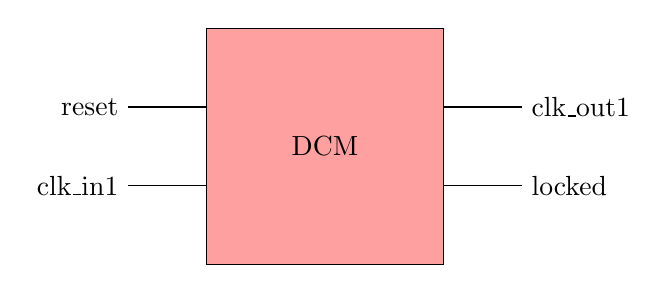
\begin{tikzpicture}
  \draw[fill=blockColor] (0,0) rectangle node{DCM}(3,3);
  \draw (-1,1) node[left]{clk\_in1}-- (0,1);
  \draw (-1,2) node[left]{reset}-- (0,2);
  \draw (4,2) node[right]{clk\_out1}-- (3,2);
  \draw (4,1) node[right]{locked}-- (3,1);
\end{tikzpicture}
\caption{Schéma bloc}
\label{dcmBloc}
\end{wrapfigure}

La norme VGA utilise une fréquence de 40MHz pour le balayage de l’écran. Or,
l’horloge intégrée à notre carte dispose d’une fréquence de 100MHz. Le bloc DCM
crée une horloge de 40MHz grâce à une horloge d'entrée de 100MHz.
Ce type de montage étant très courant, il existe des outils, appelé IP Core,
pour générer des composants génériques tels qu'un \emph{DCM}. 
\vspace{.4in}

\subsection{Entrées \& Sorties}
\label{subsec:Entrees_Sorties_dmc}

\begin{descr}
  \itemColor{reset} Reset du circuit, actif à l'état haut.
  \itemColor{clk\_in1} Horloge 100MHz, active sur front montant.
  \itemColor{clk\_out1} Horloge 40MHz.
  \itemColor{locked} Sortie non utilisée.
\end{descr}


\subsection{Problèmes rencontrés}
\label{subsec:Problemes_rencontres_dcm}

Toutes les générations d'éléments aléatoires sont basées sur la lecture d’un
compteur. Pour éviter que des séquences prédictibles puissent apparaitre, nous
avons choisi d'utiliser l'horloge à 100MHz de la FPGA en lieu et place de celle
à 40MHz générée par le bloc \emph{Digital Clock Management}. Néanmoins, lorsque
nous avons affecté le signal \emph{fpga\_clk} à l'un de nos composants (excepté
le bloc \emph{DCM}), le code n'était plus synthétisable.

Pour contourner cet étrange problème, nous avons tenté d'ajouter une sortie au
composant \emph{DCM} se contentant de copier l'horloge d'entrée sur une deuxième
horloge de sortie. Pour des raisons inconnues, le problème a persisté et le code
n'était à nouveau plus synthétisable. De ce fait, la génération d'éléments
aléatoire a, à partir de ce moment, été généré par des compteurs utilisant
l'horloge de 40MHz, mais étant réinitialisé à leur valeur maximale modulo
\emph{shipPosition}. Ce dernier signal étant la position entre le bord de
l'écran et le vaisseau du joueur, il n'est pas possible de prédire sa valeur et
cela permet d'éviter que l'aléatoire du jeu soit biaisé.

\begin{lstlisting}[style=vhdl, caption=Génération d'aléatoire]
  signal counter : integer range 0 to counterMaxValue := 0;
  
  process
  begin
    if reset = '1' then
      counter <= counterMaxValue mod shipPosition;
    elsif rising_edge(clk) then
      if counter = counterMaxValue then
        counter <= counterMaxValue mod shipPosition;
      else
        counter <= counter + 1;
      end if;
    end if;
  end process;

  -- Later in the code
  case counter is
    when 0 =>
      -- ...
\end{lstlisting}

\clearpage

\section{Display}
\label{sec:display}

\begin{wrapfigure}[30]{r}{.6\textwidth}
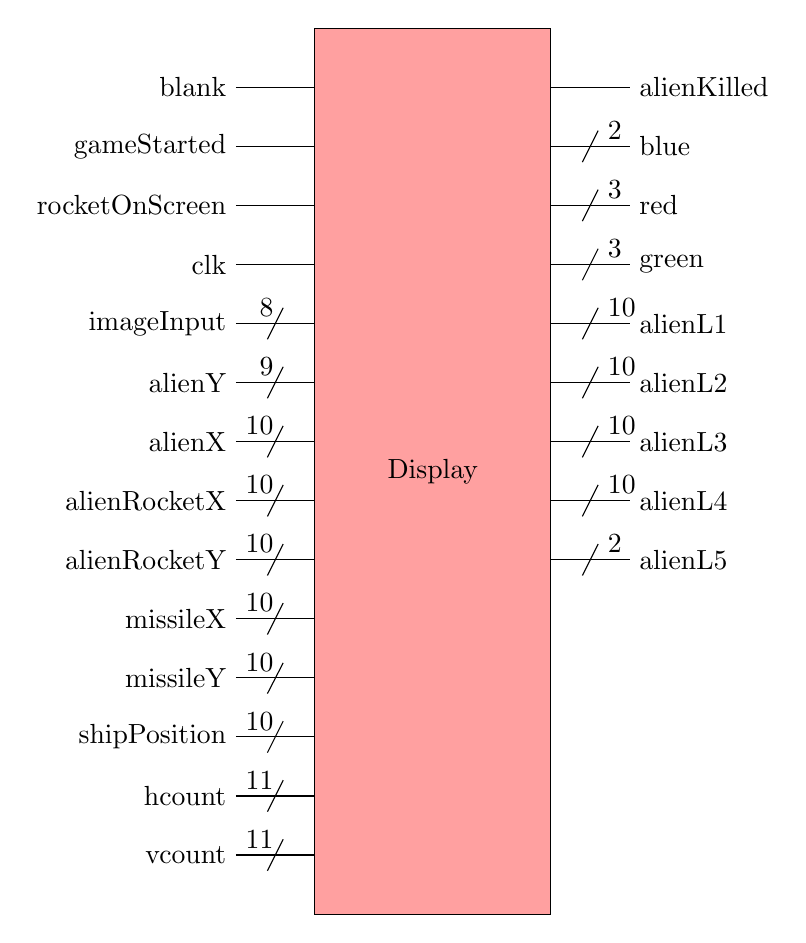
\begin{tikzpicture}
  \draw[fill=blockColor] (0,0) rectangle node{Display}(3,-11.25);
  % Inputs
  \draw (-1,-.75) node[left]{blank}-- (0,-.75);
  \draw (-1,-1.5) node[left]{gameStarted}-- (0,-1.5);
  \draw (-1,-2.25) node[left]{rocketOnScreen}-- (0,-2.25);
  \draw (-1,-3) node[left]{clk}-- (0,-3);
  \draw (-1,-3.75) node[left]{imageInput}-- (0,-3.75);
  \draw (-.4,-3.55) node[left]{8} -- (-.6, -3.95);
  \draw (-1,-4.5) node[left]{alienY}-- (0,-4.5);
  \draw (-.4,-4.3) node[left]{9} -- (-.6, -4.7);
  \draw (-1,-5.25) node[left]{alienX}-- (0,-5.25);
  \draw (-.4,-5.05) node[left]{10} -- (-.6, -5.45);
  \draw (-1,-6) node[left]{alienRocketX}-- (0,-6);
  \draw (-.4,-5.8) node[left]{10} -- (-.6, -6.2);
  \draw (-1,-6.75) node[left]{alienRocketY}-- (0,-6.75);
  \draw (-.4,-6.55) node[left]{10} -- (-.6, -6.95);
  \draw (-1,-7.5) node[left]{missileX}-- (0,-7.5);
  \draw (-.4,-7.3) node[left]{10} -- (-.6, -7.7);
  \draw (-1,-8.25) node[left]{missileY}-- (0,-8.25);
  \draw (-.4,-8.06) node[left]{10} -- (-.6, -8.45);
  \draw (-1,-9) node[left]{shipPosition}-- (0,-9);
  \draw (-.4,-8.8) node[left]{10} -- (-.6, -9.2);
  \draw (-1,-9.75) node[left]{hcount}-- (0,-9.75);
  \draw (-.4,-9.55) node[left]{11} -- (-.6, -9.95);
  \draw (-1,-10.5) node[left]{vcount}-- (0,-10.5);
  \draw (-.4,-10.3) node[left]{11} -- (-.6, -10.7);
  % Outputs
  \draw (4,-.75) node[right]{alienKilled}-- (3,-.75);
  \draw (4,-1.5) node[right]{blue}-- (3,-1.5);
  \draw (3.6,-1.3) node[right]{2} -- (3.4, -1.7);
  \draw (4,-2.25) node[right]{red}-- (3,-2.25);
  \draw (3.6,-2.05) node[right]{3} -- (3.4, -2.45);
  \draw (4,-3) node[right]{green}-- (3,-3);
  \draw (3.6,-2.8) node[right]{3} -- (3.4, -3.2);
  \draw (4,-3.75) node[right]{alienL1}-- (3,-3.75);
  \draw (3.6,-3.55) node[right]{10} -- (3.4, -3.95);
  \draw (4,-4.5) node[right]{alienL2}-- (3,-4.5);
  \draw (3.6,-4.3) node[right]{10} -- (3.4, -4.7);
  \draw (4,-5.25) node[right]{alienL3}-- (3,-5.25);
  \draw (3.6,-5.05) node[right]{10} -- (3.4, -5.45);
  \draw (4,-6) node[right]{alienL4}-- (3,-6);
  \draw (3.6,-5.8) node[right]{10} -- (3.4, -6.2);
  \draw (4,-6.75) node[right]{alienL5}-- (3,-6.75);
  \draw (3.6,-6.55) node[right]{2} -- (3.4, -6.95);
\end{tikzpicture}
\caption{Schéma bloc}
\label{displayBloc}
\end{wrapfigure}

Grâce aux signaux générés par les composants \emph{VGA\_Internal} et
\emph{DCM}, \emph{Display} est en mesure d'afficher des données à l'écran au
moyen des trois sorties \emph{red}, \emph{green} et \emph{blue}. Ces dernières
sont codées sur trois bits, à l'exception de la composante bleue qui n'est constituée que de deux bits, en accord avec la norme VGA.

Différents tests sont effectués dans \emph{Display} pour distinguer quels éléments
doivent être affichés et lesquels ne doivent pas l'être. Le premier d'entre eux,
est de consulter la valeur de \emph{gameStarted} pour afficher ou non l'écran
titre du jeu. Si cette valeur vaut 1, le composant détecte si la partie est
terminée ou encore en cours. Pour cela, il suffit de regarder si la roquette des
aliens est aux même coordonnées que le vaisseau du joueur.

De cette manière, \emph{Display} est non seulement utilisé pour afficher des
données à l'écran, mais également pour faire des tests sur l'état du jeu, comme
la détection de fin de partie (que ce soit une victoire ou une défaite du
joueur) ainsi que la gestion des collisions entre les roquettes et les aliens ou
le joueur. Le choix d'avoir fait ces tests à l'intérieur de \emph{Display} plutôt
que de créer un nouveau bloc spécifique à ce cas fut dirigé par le fait que
tous les signaux nécessaires à ces deux tests étaient déjà présents dans ce
bloc, et qu'il aurait été redondant de les ajouter ailleurs.

\begin{wrapfigure}[14]{l}{.5\textwidth}
\lstinputlisting[style=vhdl, firstline=423, lastline=435, caption=Détection de
la mort du joueur.]{../Development/v1.5/Display.vhd}
\end{wrapfigure}

Lorsque la partie est en cours, les aliens sont affichés à l'écran selon les
signaux internes \emph{alienLine1} à \emph{alienLine5}. Ces derniers
fonctionnent de la même manière que dans le bloc \emph{alienRocket} (voir
tableau \ref{alientable}).

Ci-contre se trouve le code permettant de détecter la collision entre un tir
alien et le spationef. Ce dernier a une hauteur de 30 pixels, pour une largeur
de 62 pixels. De ce fait, lorsqu'une roquette a sa position en $Y$ entre 570
et 600 et que sa position en $X$ est entre la position du vaisseau et cette
dernière $+ 56$, le joueur s'est fait toucher.

Le range $X$ du vaisseau est calculé entre $\emph{shipPosition}+6$ et
$\emph{shipPosition}+56$ pour supprimer, de la détection, les 6 pixels noirs
présent de chaque côté du spationef.


\clearpage

\subsection{Entrées \& Sorties}
\label{subsec:Entrees_Sorties_display}

\begin{descr}
  \itemColor{blank} Si 1, le balayage est en dehors de l'écran et les
  composantes RGB, c'est-à-dire les sorties \emph{red}, \emph{blue} et
  \emph{green} doivent être nul.
  \itemColor{gameStarted} Indique par une valeur à 1 que le jeu à débuté.
  \itemColor{rocketOnScreen} Indique par une valeur à 1 qu'une roquette doit être
  affiché à l'écran.
  \itemColor{clk} Horloge 40MHz, active sur front montant.
  \itemColor{imageInput} Bus de données en provenance de la ROM contenant
  l'image d'accueil du jeu.
  \itemColor{alienY} Nombre de pixels entre le haut de l'écran et le bord
  supérieur des aliens contenus dans \emph{alienLine1}.
  \itemColor{alienX} Nombre de pixels entre le bord gauche de l'écran et le
  bord droit des aliens à l'index 0.
  \itemColor{alienRocketX} Nombre de pixels entre le bord gauche de l'écran et
  la roquette tirée par les aliens.
  \itemColor{alienRocketY} Nombre de pixels entre le le haut de l'écran et le
  haut de la rockette tirée par les aliens.
  \itemColor{missileX} Nombre de pixels entre le bord gauche de l'écran et la roquette
  lancée par les aliens.
  \itemColor{missileY} Nombre de pixels entre le haut de l'écran et le haut de la rockette
  lancée par les aliens.
  \itemColor{shipPosition} Nombre de pixels entre le bord gauche de l'écran et
  le bord gauche du vaisseau contrôlé par le joueur.
  \itemColor{hcount} Coordonnée $X$ du balayage.
  \itemColor{vcount} Coordonnée $Y$ du balayage.
  \itemColor{alienKilled} Indique par une valeur à 1 qu'un alien a été touché
  par une rockette lancée par le joueur.
  \itemColor{blue} Composante bleue de la sortie VGA.
  \itemColor{red} Composante rouge de la sortie VGA.
  \itemColor{green} Composante verte de la sortie VGA.
  \itemColor{alienL1} Indique par une valeur à 1 la présence d'un alien au même
  index dans la rangée d'aliens la plus proche du haut de l'écran (voir tableau
  \ref{alientable}).
  \itemColor{alienL2} Identique à \emph{alienL1} pour la rangée d'aliens inférieur.
  \itemColor{alienL3} Identique à \emph{alienL2} pour la rangée d'aliens inférieur.
  \itemColor{alienL4} Identique à \emph{alienL3} pour la rangée d'aliens inférieur.
  \itemColor{alienL5} Identique à \emph{alienL4} pour la rangée d'aliens inférieur.
\end{descr}

\clearpage

\section{Input}
\label{sec:input}


\begin{wrapfigure}[16]{l}{.6\textwidth}
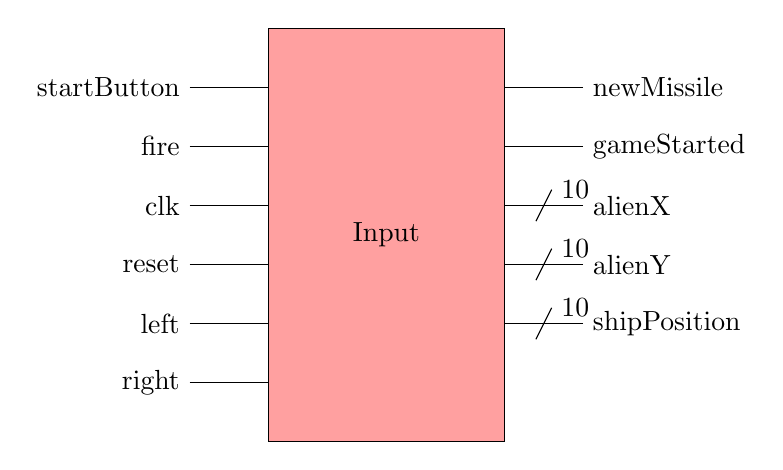
\begin{tikzpicture}
  \draw[fill=blockColor] (0,0) rectangle node{Input}(3,-5.25);
  % Inputs
  \draw (-1,-.75) node[left]{startButton} -- (0,-.75);
  \draw (-1,-1.5) node[left]{fire}-- (0,-1.5);
  \draw (-1,-2.25) node[left]{clk}-- (0,-2.25);
  \draw (-1,-3) node[left]{reset}-- (0,-3);
  \draw (-1,-3.75) node[left]{left}-- (0,-3.75);
  \draw (-1,-4.5) node[left]{right}-- (0,-4.5);
  % Outputs
  \draw (4,-.75) node[right]{newMissile}-- (3,-.75);
  \draw (4,-1.5) node[right]{gameStarted}-- (3,-1.5);
  \draw (4,-2.25) node[right]{alienX}-- (3,-2.25);
  \draw (3.6,-2.05) node[right]{10} -- (3.4, -2.45);
  \draw (4,-3) node[right]{alienY}-- (3,-3);
  \draw (3.6,-2.8) node[right]{10} -- (3.4, -3.2);
  \draw (4,-3.75) node[right]{shipPosition}-- (3,-3.75);
  \draw (3.6,-3.55) node[right]{10} -- (3.4, -3.95);
\end{tikzpicture}
\caption{Schéma bloc}
\label{inputBloc}
\end{wrapfigure}

\emph{Input} est chargé de recevoir et traiter les actions faites par le joueur.
Via quatre des cinq boutons de la croix directionnelle, le joueur peut démarrer
une partie, déplacer son vaisseau et tirer. Toutes ses actions sont traiter dans
\emph{Input}, tout comme le déplacement aléatoire des aliens sur l'écran. Ces
derniers peuvent se mouvoir en haut, bas, gauche, droite ainsi qu'en diagonale.
La direction qu'ils prennent est aléatoire, en fonction d'un compteur
\emph{alienDirection} s'incrémentant à chaque coût d'horloge. De plus, la
distance, ou saut, qu'ils parcourent en un déplacement est également aléatoire
via un autre compteur \emph{alienJump}. La taille maximale d'un saut peut être
définie en modifiant la valeur \emph{maxAlienJump} dans le package du jeu.

\lstinputlisting[style=vhdl, caption=Déplacement des aliens]{vhdl/alienDirection.vhd}

\subsection{Entrées \& Sorties}
\label{subsec:Entrees_Sorties_input}

\begin{descr}
  \itemColor{startButton} Bouton situé au centre de la croix directionnelle (B8).
  Utilisé pour démarrer une partie depuis l'écran d'accueil.
  \itemColor{fire} Bouton supérieur de la croix directionnelle (BTNU, A8).
  Utilisé pour tirer des lasers depuis le vaisseau vers les aliens pendant une partie.
  \itemColor{clk} Horloge 40MHz, active sur front montant.
  \itemColor{reset} Reset du circuit, actif à l'état haut.
  \itemColor{left} Bouton gauche de la croix directionnelle (BTNL, C4). Utilisé
  pour déplacer le vaisseau du joueur vers la gauche.
  \itemColor{right} Bouton droit de la croix directionnelle (BTNR, D9). Utilisé
  pour déplacer le vaisseau du joueur vers la droite.
  \itemColor{newMissile} Indique par une valeur à 1 qu'un nouveau missile a été
  tiré par le vaisseau du joueur.
  \itemColor{gameStarted} Indique par une valeur à 1 que le jeu à débuté.
  \itemColor{alienX} Nombre de pixels entre le bord gauche de l'écran et le
  bord droit des aliens à l'index 0.
  \itemColor{alienY} Nombre de pixels entre le haut de l'écran et le bord
  supérieur des aliens contenus dans \emph{alienLine1}.
  \itemColor{shipPosition} Nombre de pixels entre le bord gauche de l'écran et
  le bord droit du vaisseau de joueur. Cette valeur est utilisée pour générer de l'aléatoire.
\end{descr}

\subsection{Testbench}
\label{subsec:Testbench_input}

\lstinputlisting[style=vhdl, caption=InputTestbench.]{../TestBenchs/InputTestBench.vhd}

\clearpage

\section{rocketManager}
\label{sec:rocketmanager}

\begin{wrapfigure}[14]{r}{.6\textwidth}
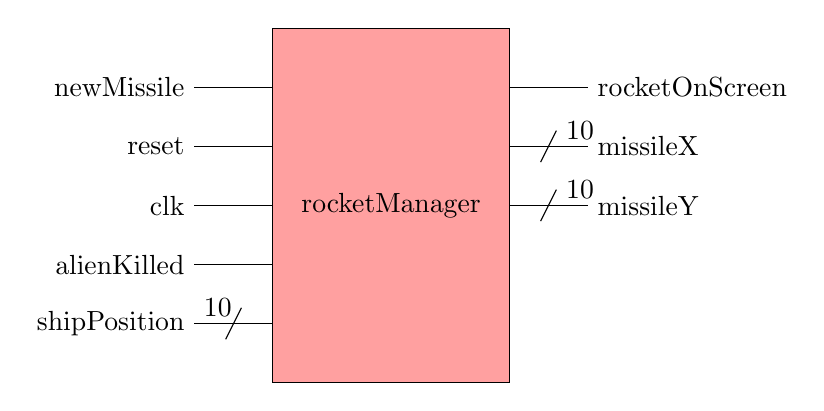
\begin{tikzpicture}
  \draw[fill=blockColor] (0,0) rectangle node{rocketManager}(3,-4.5);
  % Inputs
  \draw (-1,-.75) node[left]{newMissile}-- (0,-.75);
  \draw (-1,-1.5) node[left]{reset}-- (0,-1.5);
  \draw (-1,-2.25) node[left]{clk}-- (0,-2.25);
  \draw (-1,-3) node[left]{alienKilled}-- (0,-3);
  \draw (-1,-3.75) node[left]{shipPosition}-- (0,-3.75);
  \draw (-.4,-3.55) node[left]{10} -- (-.6, -3.95);
  % Outputs
  \draw (4,-.75) node[right]{rocketOnScreen}-- (3,-.75);
  \draw (4,-1.5) node[right]{missileX}-- (3,-1.5);
  \draw (3.6,-1.3) node[right]{10} -- (3.4, -1.7);
  \draw (4,-2.25) node[right]{missileY}-- (3,-2.25);
  \draw (3.6,-2.05) node[right]{10} -- (3.4, -2.45);
\end{tikzpicture}
\caption{Schéma bloc}
\label{rocketManagerBloc}
\end{wrapfigure}

Le bloc \emph{rocketManager} a pour rôle de générer les missiles du vaisseau
spatial que le joueur pilote. Le bloc \emph{Input} fourni à \emph{rocketManager}
une impulsion, via le signal \emph{newMissile}, lorsque celui-ci doit générer un
nouveau missile. Cette impulsion apparaît lorsque le jour clique sur le bouton
pour tirer un nouveau missile. Dès qu'un missile est tiré (\emph{fire}), celui-ci doit avoir
une coordonnée en X, une coordonnée en Y ainsi qu'être signalé au bloc
\emph{Display} afin que celui-ci sache qu'un missile doit être affiché.

L'entrée \emph{alienKilled} permet au bloc de savoir si un alien a été touché,
et dans ce cas le signal de sortie \emph{rocketOnScreen} passera à 0 et le
missile n'apparaîtra plus à l'écran. Ce signal passe
également à 0 lorsque le missile atteint le haut de l'écran.

\emph{RocketManager} utilise le signal \emph{shipPosition}, qui correspond à la
coordonnée sur l'axe horizontal du vaisseau au moment du tir, afin de fournir
en sortie (\emph{missileX}) la position X du missile. Cette position reste la
même tant que le missile n'a pas atteint un alien ou le haut de l'écran.

Concernant la position Y du missile, celle-ci se comporte comme un compteur. En
effet, cette position est remise à la valeur de 570 (hauteur de l'écran moins la
hauteur du vaisseau), afin que le missile parte du vaisseau, et est ensuite
décrémentée jusqu'à la valeur minimale de 0 (le missile atteint donc le haut de
l'écran).

Les positions X et Y sont fournis au bloc \emph{Display} via leurs signaux
respectifs et ce dernier se charge d'afficher le missile.

Le bloc \emph{rocketManager} utilise l’horloge afin de décrémenter le compteur de
la position Y et le signal reset afin de remettre tous les signaux dans leur
état d'origine.

\subsection{Entrées \& Sorties}
\label{subsec:Entrees_Sorties_rocketManager}

\begin{descr}
  \itemColor{newMissile} Indique par une valeur à 1 qu'un nouveau missile a été
  tiré par le vaisseau du joueur.
  \itemColor{reset} Reset du circuit, actif à l'état haut.
  \itemColor{clk} Horloge 40MHz, active sur front montant.
  \itemColor{alienKilled} Indique par une valeur à 1 qu'un alien a été touché
  par une roquette lancée par le joueur.
  \itemColor{shipPosition} Nombre de pixels entre le bord gauche de l'écran et
  le bord droit du vaisseau de joueur. Cette valeur est utilisée pour générer de l'aléatoire.
  \itemColor{rocketOnScreen} Indique par une valeur à 1 qu'une roquette doit être
  affiché à l'écran.
  \itemColor{missileX} Nombre de pixels entre le bord gauche de l'écran et la roquette
  lancée par les aliens.
  \itemColor{missileY} Nombre de pixels entre le haut de l'écran et le haut de la roquette
  lancée par les aliens.
\end{descr}
\clearpage

\subsection{Testbench}
\label{subsec:Testbench_rocketManager}

\lstinputlisting[style=vhdl, firstline=20, caption=RocketManagerTestbench.]{../TestBenchs/RocketManagerTestBench.vhd}

\clearpage

\section{VGA Internal}
\label{sec:vgainternal}


\begin{wrapfigure}[14]{l}{.5\textwidth}
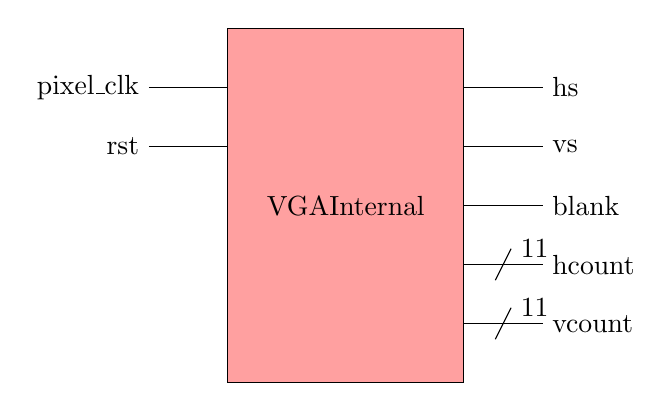
\begin{tikzpicture}
  \draw[fill=blockColor] (0,0) rectangle node{VGAInternal}(3,-4.5);
  % Inputs
  \draw (-1,-.75) node[left]{pixel\_clk} -- (0,-.75);
  \draw (-1,-1.5) node[left]{rst}-- (0,-1.5);
  % Outputs
  \draw (4,-.75) node[right]{hs}-- (3,-.75);
  \draw (4,-1.5) node[right]{vs}-- (3,-1.5);
  \draw (4,-2.25) node[right]{blank}-- (3,-2.25);
  \draw (4,-3) node[right]{hcount}-- (3,-3);
  \draw (3.6,-2.8) node[right]{11} -- (3.4, -3.2);
  \draw (4,-3.75) node[right]{vcount}-- (3,-3.75);
  \draw (3.6,-3.55) node[right]{11} -- (3.4, -3.95);
\end{tikzpicture}
\caption{Schéma bloc}
\label{vgaInternalBloc}
\end{wrapfigure}

Une interface VGA fonctionne selon les trois composantes RGB ainsi qu’une
synchronisation horizontale et verticale. Les signaux RGB décrivent
la couleur des pixels composant l’image selon un balayage effectué de gauche à
droite, en ligne de haut en bas. L’écran recevant ce flux RGB est capable de
savoir à quel pixel il correspond selon l’instant $t$ auquel il lit ces données
dans le balayage. Néanmoins, ce n’est pas l’écran qui est chargé de sauter
automatiquement à la ligne suivante lorsque chaque pixel de la ligne actuel a
été traité. C’est ce à quoi sert le signal \emph{HS}, alors que \emph{VS} indique un retour à
la première ligne.\\

\infoInfo{Retour à la ligne}{Afin d’informer le moniteur que le
balayage est arrivé à la fin d’une ligne et que le prochain pixel sera le premier de
la ligne suivante, le signal HS produit une impulsion
de synchronisation. De même, lorsque le balayage est
arrivé à la fin de la dernière ligne (et donc que toute
une image a été transmise), le signal VS produit une impulsion pour indiquer un
retour à la première ligne (et donc la transmission d’une nouvelle image).}

Lorsque le balayage se trouve en dehors de l'écran, le signal \emph{blank} prend
comme valeur 0 afin d'indiquer au bloc \emph{Display} de mettre les composantes
de sorties RGB à 0. Ce comportement est défini dans la norme VGA et résulte
dans une erreur d'affichage ``Index out of bound'' s'il n'est pas respecté.

\subsection{Entrées \& Sorties}
\label{subsec:Entrees_Sorties_vga}

\begin{descr}
  \itemColor{pixel\_clk} Horloge 40MHz, active sur front montant.
  \itemColor{rst} Reset du circuit, actif à l'état haut.
  \itemColor{hs} Impulsion de synchronisation horizontale. Indique par une pulse
  à l'état haut un retour à la ligne du balayage de l'écran.
  \itemColor{vs} Impulsion de synchronisation verticale. Indique par une pulse à
  l'état haut un retour du balayage à la première ligne de l'écran.
  \itemColor{blank} Si 1, le balayage est en dehors de l'écran et les
  composantes RGB, c'est-à-dire les sorties \emph{red}, \emph{blue} et
  \emph{green} doivent être nul.
  \itemColor{hcount} Coordonnée $X$ du balayage.
  \itemColor{vcount} Coordonnée $Y$ du balayage.
\end{descr}

\clearpage

\section{Top Module}
\label{sec:topmodule}

\begin{wrapfigure}[14]{r}{.5\textwidth}
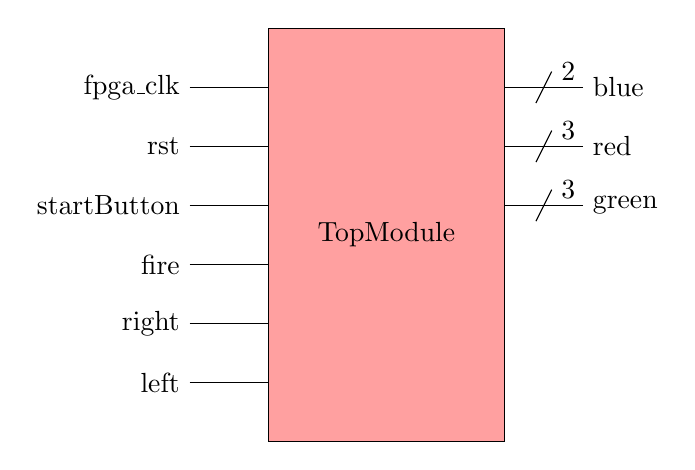
\begin{tikzpicture}
  \draw[fill=blockColor] (0,0) rectangle node{TopModule}(3,-5.25);
  % Inputs
  \draw (-1,-.75) node[left]{fpga\_clk}-- (0,-.75);
  \draw (-1,-1.5) node[left]{rst}-- (0,-1.5);
  \draw (-1,-2.25) node[left]{startButton}-- (0,-2.25);
  \draw (-1,-3) node[left]{fire}-- (0,-3);
  \draw (-1,-3.75) node[left]{right}-- (0,-3.75);
  \draw (-1,-4.5) node[left]{left}-- (0,-4.5);
  % Outputs
  \draw (4,-.75) node[right]{blue}-- (3,-.75);
  \draw (3.6,-.55) node[right]{2} -- (3.4, -.95);
  \draw (4,-1.5) node[right]{red}-- (3,-1.5);
  \draw (3.6,-1.3) node[right]{3} -- (3.4, -1.7);
  \draw (4,-2.25) node[right]{green}-- (3,-2.25);
  \draw (3.6,-2.05) node[right]{3} -- (3.4, -2.45);
\end{tikzpicture}
\caption{Schéma bloc}
\label{topModuleBloc}
\end{wrapfigure}


Le bloc \emph{topModule} est comme son nom l'indique l'élément tout en haut de notre architecture. Il instancie les composants et relie ceux-ci via des signaux intermédiaires. 

Concernant ses entrées et sorties, celles-ci sont des éléments physiques de la carte FPGA et sont assignées via le fichier UCF. Le signal d'entrée \emph{fpga\_clk} correspond à l’horloge de la FPGA. Cette horloge fonctionne à une fréquence de 100 MHz. Le \emph{reset} est assigné sur le switch SW8 (figure \ref{motherboard}) et permet le reset software du jeu.

Plusieurs boutons sont utilisés afin de jouer et ont donc été assignés grâce au fichier UCF. Au niveau des signaux, il s'agit de \emph{startButton}, de \emph{fire}, de \emph{right} et de \emph{left}. 
Le bouton \emph{fire} permet de tirer un missile depuis le vaisseau. Puisqu'il n'est possible que de tirer un seul missile à la fois, celui-ci n'a pas d'effet tant qu'il y a un missile en déplacement. 
Les boutons \emph{right} et \emph{left} sont explicites. Ils permettent le déplacement latéral du vaisseau que pilote le joueur.
Le \emph{startButton} permet de passer de l'écran de démarrage au jeu. Il n'a d'effet que durant cette étape afin qu'en cas d'appui involontaire durant la partie celle-ci ne s'en retrouve pas impactée.

Nous avions commencé par utiliser un seul bouton afin de passer de l'écran de démarrage au jeu et pour tirer des missiles. Cependant, lorsque le jeu commençait, un missile était automatiquement tiré et cela ne correspondait pas à ce que nous voulions. Nous avons cherché un moyen de corriger ce problème, mais cela s'est avéré compliqué pour un problème mineur alors qu'une solution simple, et finalement plus pratique, était de séparer ces deux fonctions en deux boutons.

Concernant les sorties \emph{blue}, \emph{red} et \emph{green}, celles-ci sont assignées sur la sortie VGA de la carte. Ces signaux correspondent aux trois couleurs (RGB) utilisées par le VGA afin d'afficher sur un écran. Puisque le VGA utilise 8 bits, les signaux \emph{red} et \emph{green} disposent de 3 bits chacun. Le signal \emph{blue} ne dispose que de 2 bits.
Il est tout de même possible d'afficher 256 couleurs différentes.

\subsection{Entrées \& Sorties}
\label{subsec:Entrees_Sorties_topModule}

\begin{descr}
  \itemColor{fpga\_clk} Horloge 100MHz, active sur front montant.
  \itemColor{rst} Reset du circuit, actif à l'état haut.
  \itemColor{startButton} Bouton situé au centre de la croix directionnelle (B8).
  Utilisé pour démarrer une partie depuis l'écran d'accueil.
  \itemColor{fire} Bouton supérieur de la croix directionnelle (BTNU, A8). Tire des lasers sur les aliens.
  \itemColor{right} Bouton droit de la croix directionnelle (BTNR, D9). Déplace le vaisseau à droite.
  \itemColor{left} Bouton gauche de la croix directionnelle (BTNL, C4). Déplace le vaisseau à gauche.
  \itemColor{blue} Composante bleue de la sortie VGA.
  \itemColor{red} Composante rouge de la sortie VGA.
  \itemColor{green} Composante verte de la sortie VGA.
\end{descr}

\clearpage

\subsection{Architecture}
\label{sub:architecture}

\begin{figure}[h!]
   \centering
   \includegraphics[width=\textwidth,height=.9\textheight]{pictures/TopModuleArchitecture}
\end{figure}

\clearpage


\section{Space Invaders Package}
\label{sec:package}

Généralement, il est recommandé de programmer en utilisant des variables et non
des \emph{Magic Numbers} dans les langages de programmation dits
``haut-niveau''. Les performances du code ne seront que peu, voir pas du tout
impacté selon la qualité du compilateur. En revanche, le programme sera plus
compréhensible dans le cas d'un débogage ou d'un changement de programmeur.

Autre avantage, modifier une variable à un seul endroit fera le changement dans
l'ensemble du code sans qu'il n'y ait de risques d'erreurs humaines, tel que
modifier le mauvais nombre car deux \emph{Magic Numbers} différents avaient la
même valeur.

En VHDL, il est également recommandé de programmer selon ce principe. Néanmoins,
un composant VHDL ne peut transmettre d'information à un autre sans qu'un signal
contenant les données à partager soit implémenté entre les deux blocs. Lorsqu'un
programme contient de nombreuses variables dites génériques, ces dernières peuvent
rapidement rendre le design schématique du projet incompréhensible en ajoutant
énormément de connexions entre les blocs.

Une solution à cette problématique est l'utilisation de \emph{package}. Un
\emph{package} peut être lu et modifié par n'importe quel composant l'ayant
importé.
\begin{lstlisting}[style=vhdl, caption=Importation d'un package]
library work;
use work.SpaceInvadersPackage.all;
\end{lstlisting}

Par défaut, un package est contenu dans la libraire \emph{work}, qui doit donc
également être importée. Notre jeu est codé en utilisant au maximum des signaux
contenus dans un package, qui peuvent être modifiés pour changer certains
paramètres du jeu.

\begin{lstlisting}[style=vhdl, caption=Signaux utilisés par \emph{Input} \& \emph{rocketManager}]
-- Inputs
  constant fireSpeed        : integer                      := 600000;
  constant shipSpeed        : integer                      := 100000;
  constant alienSpeed       : integer                      := 6000000;
  constant maxShipPosValue  : integer                      := 736;  -- must be pair
  constant shipMargin       : integer                      := 50;   -- minimum space between side screen and ship
  constant alienXMargin     : integer                      := 50;   -- minimum space between side screen and aliens
  constant alienYUpMargin   : integer                      := 50;   -- minimum space between top screen and aliens
  constant alienYDownMargin : integer                      := 200;  -- maximum space between top screen and aliens
  constant maxAlienJump     : integer                      := 10;   -- max pixel
  aliens can shift in a single time
  ---------------------------------------------------------------------------------------------------------------
-- rocketManager
  constant missileSpeed     : integer                      := 60000;  -- missile speed
  constant rocketLength     : integer                      := 10;     -- rocket length in pixel
  constant rocketColor      : std_logic_vector(7 downto 0) := "11111111";
\end{lstlisting}

Admettons que l'on souhaite modifier la couleur des roquettes, il suffit de changer la valeur de \emph{rocketColor} pour que ce
changement soit effectué dans tous les composants nécessaires. 

\asymmetricalPage
\chapter{Annexes}

\symmetricalPage

\section{Convertion d'image}
\label{sec:convertPicture}

Le bloc \emph{Display} affiche des données à l'écran en affectant une valeur aux
trois signaux \emph{red}, \emph{green} et \emph{blue}. Les deux premiers sont
contenus sur trois bits, alors que le dernier est uniquement sur deux. Cela
signifie que le jeu de couleurs à disposition vaut:
\begin{align*}
  n_{colors} &= 2^{8}\\
             &= 256
\end{align*}

Une couleur est ainsi affectée à chaque pixel, en commençant par celui en haut à
gauche de l'écran, puis celui à sa droite et ainsi de suite jusqu'à arriver à la
droite de l'écran et commencer la ligne suivante. Il apparait alors que pour
afficher une image, il faut extraire le code couleur de chacun de ses pixels,
puis les stocker d'une des deux façons suivantes:\vspace{.1in}
\begin{items}
\item Dans une RAM ou une ROM, cela implique de convertir l'image en un fichier
  \emph{COE} de la forme suivante:
  \begin{lstlisting}[frame=single, basicstyle=\scriptsize, backgroundcolor=\color{backcolor}]
memory_initialization_radix=16;
memory_initialization_vector=
43,
26,
2,
6e,
6e,
4a,
d9,
b6,
6e,
dd,
b5,
6a,
dd,
b6,
6a;
\end{lstlisting}
\emph{memory\_initialization\_radix=16;} indique les valeurs sont stockées en
hexadécimale. Il est possible de le faire en binaire ou en décimal.
\vspace{.1in}
\item Dans un tableau 2D:
  \begin{lstlisting}[style=vhdl]
type memoryPicture is array(0 to 4, 0 to 2) of integer;
constant picture : memoryPicture:=(
(16#43#,16#26#,16#2#),
(16#6e#,16#6e#,16#4a#),
(16#d9#,16#b6#,16#6e#),
(16#dd#,16#b5#,16#6a#),
(16#dd#,16#b6#,16#6a#));
  \end{lstlisting}
\end{items}

Avec un COE, chaque valeur est stockée à la suite. En utilisant un tableau VHDL,
il est possible de stocker en deux dimensions les valeurs pour avoir une
représentation identique à celle de l'écran. La forme \emph{16\#<value>\#} indique
en VHDL que le nombre est sous forme hexadécimale et peut être directement
assigné à un signal de type sdl\_logic\_vector.

Afin de rapidement convertir des images en fichier COE ou en tableau 2D VHDL,
nous avons écrit un script Matlab. Le détail de son fonctionnement est inclus
dans les commentaires du code.

\infoInfo{Format des images}{Seules les images au format ``JPG'' sont supportées
  par le script.}

\clearpage

\subsection{Script Matlab - Convertion en fichier COE}
\label{subsec:Script1}
\vspace{.1in}
\lstinputlisting[style=matlab]{matlab/picturesToCOE.m}
\clearpage

\subsection{Script Matlab - Convertion en tableau VHDL}
\label{subsec:Script2}
\vspace{.1in}
\lstinputlisting[style=matlab]{matlab/picturesToFPGA.m}

\clearpage

\section{Code source}
\label{sec:code}

\subsection{alienRocket}
\lstinputlisting[style=vhdl]{../Development/v1.5/alienRocket.vhd}

\clearpage
\subsection{Digital Clock Management}
\lstinputlisting[style=vhdl]{vhdl/dcm.vhd}
\clearpage
\subsection{Display}
\lstinputlisting[style=vhdl]{../Development/v1.5/Display.vhd}
\clearpage
\subsection{Input}
\lstinputlisting[style=vhdl]{../Development/v1.5/input.vhd}

\subsection{rocketManager}
\lstinputlisting[style=vhdl]{../Development/v1.5/rocketManager.vhd}

\subsection{VGA Internal}
\lstinputlisting[style=vhdl]{../Development/v1.5/VGA_Internal.vhd}
\clearpage
\subsection{Top Module}
\lstinputlisting[style=vhdl]{../Development/v1.5/TopModule.vhd}

\subsection{Package}
\lstinputlisting[style=vhdl, lastline=93]{../Development/v1.5/SpaceInvadersPackage.vhd}


\end{document}
